\documentclass[a4paper,11pt]{article}
% Use ctrl + alt + V to view live pdf

% Packages
\usepackage[utf8]{inputenc} % For encoding
\usepackage[T1]{fontenc} % Better handling of accented characters and hyphenation
\usepackage{microtype} % Improves spacing and justification
\usepackage{amsmath, amssymb} % For equations and symbols
\usepackage{graphicx} % For including graphics/images
\usepackage{caption} % For customizing figure and table captions
\usepackage{subcaption} % For subfigures and subcaptions
\usepackage{float} % For fixing figure and table positions
\usepackage{booktabs} % For professional-looking tables
\usepackage{siunitx} % For consistent typesetting of units and numbers
\usepackage[margin=2cm]{geometry} % Adjusts page margins
\usepackage{fancyhdr} % For custom headers and footers
\usepackage{lmodern} % For a professional-looking font (main body font)
\usepackage{titlesec} % For title customization
\usepackage{array} % For custom table formatting
\usepackage[colorlinks=true, linkcolor=black, urlcolor=black]{hyperref} % Colored links without boxes
\usepackage{cleveref} % For improved cross-referencing    
\usepackage{multirow}
\usepackage{enumitem}
\usepackage{listings}
\usepackage{xcolor}
\usepackage{textcomp}
\usepackage{tabularx}
\usepackage{changepage}
\usepackage{tikz}
\usepackage{pdfpages}
\usetikzlibrary{shapes.geometric, arrows}
\newcolumntype{Y}{>{\centering\arraybackslash}X}
% Reduce spacing before and after \section
% \titlespacing{\section}{0pt}{1.0em}{0.5em}
% Reduce spacing before and after \subsection
% \titlespacing{\subsection}{0pt}{0.8em}{0.3em}


\lstdefinestyle{vhdl-style}{
    language=VHDL,
    basicstyle=\ttfamily\footnotesize,
    keywordstyle=\bfseries\color{blue},
    commentstyle=\itshape\color{gray},
    stringstyle=\color{red},
    numbers=left,
    numberstyle=\tiny\color{gray},
    stepnumber=1,
    breaklines=true,
    showstringspaces=false,
    frame=single
}
\lstset{style=vhdl-style}
\lstset{captionpos=b}
\lstset{basicstyle=\ttfamily\scriptsize} 
\renewcommand{\lstlistingname}{Program}

% Custom settings
\pagestyle{fancy}
\fancyhf{}
\fancyhead[L]{\textit{GB3 - Risc-V Processor}} % Header left
\fancyhead[R]{\textit{Will Hewes - wh365}} % Header right 
\fancyfoot[C]{\thepage} % Footer center
\setlength{\headheight}{15pt} % Header height
\setlength{\parindent}{0em} % Indentation for paragraphs
\setlength{\parskip}{0.2em} % Add spacing between paragraphs
\setlength{\abovedisplayskip}{0.5em}
\setlength{\belowdisplayskip}{0.5em}
\setlength{\abovedisplayshortskip}{0.5em}
\setlength{\belowdisplayshortskip}{0.5em}
\setlist{topsep=0em, partopsep=0em, itemsep=0em, parsep=0em}

\graphicspath{{Images/}}

% \renewcommand{\arraystretch}{1.2}

% Title formatting
\renewcommand{\maketitle}{
    \begin{center}
        \LARGE \textbf{ENGINEERING TRIPOS PART IIA} \\ 
        \vspace{0.5em}
        \Large \textbf{GB3 - Risc-V Processor} \\ 
        \vspace{0.5em}
        \textbf{Final Report} \\
        \large Group 4 - Resource Usage \\
        \vspace{1em}
        \large Will Hewes - wh365 \\ 
        Pembroke College \\ 
        \vspace{0.5em}
    \end{center}
}

\begin{document}
\pagenumbering{gobble}
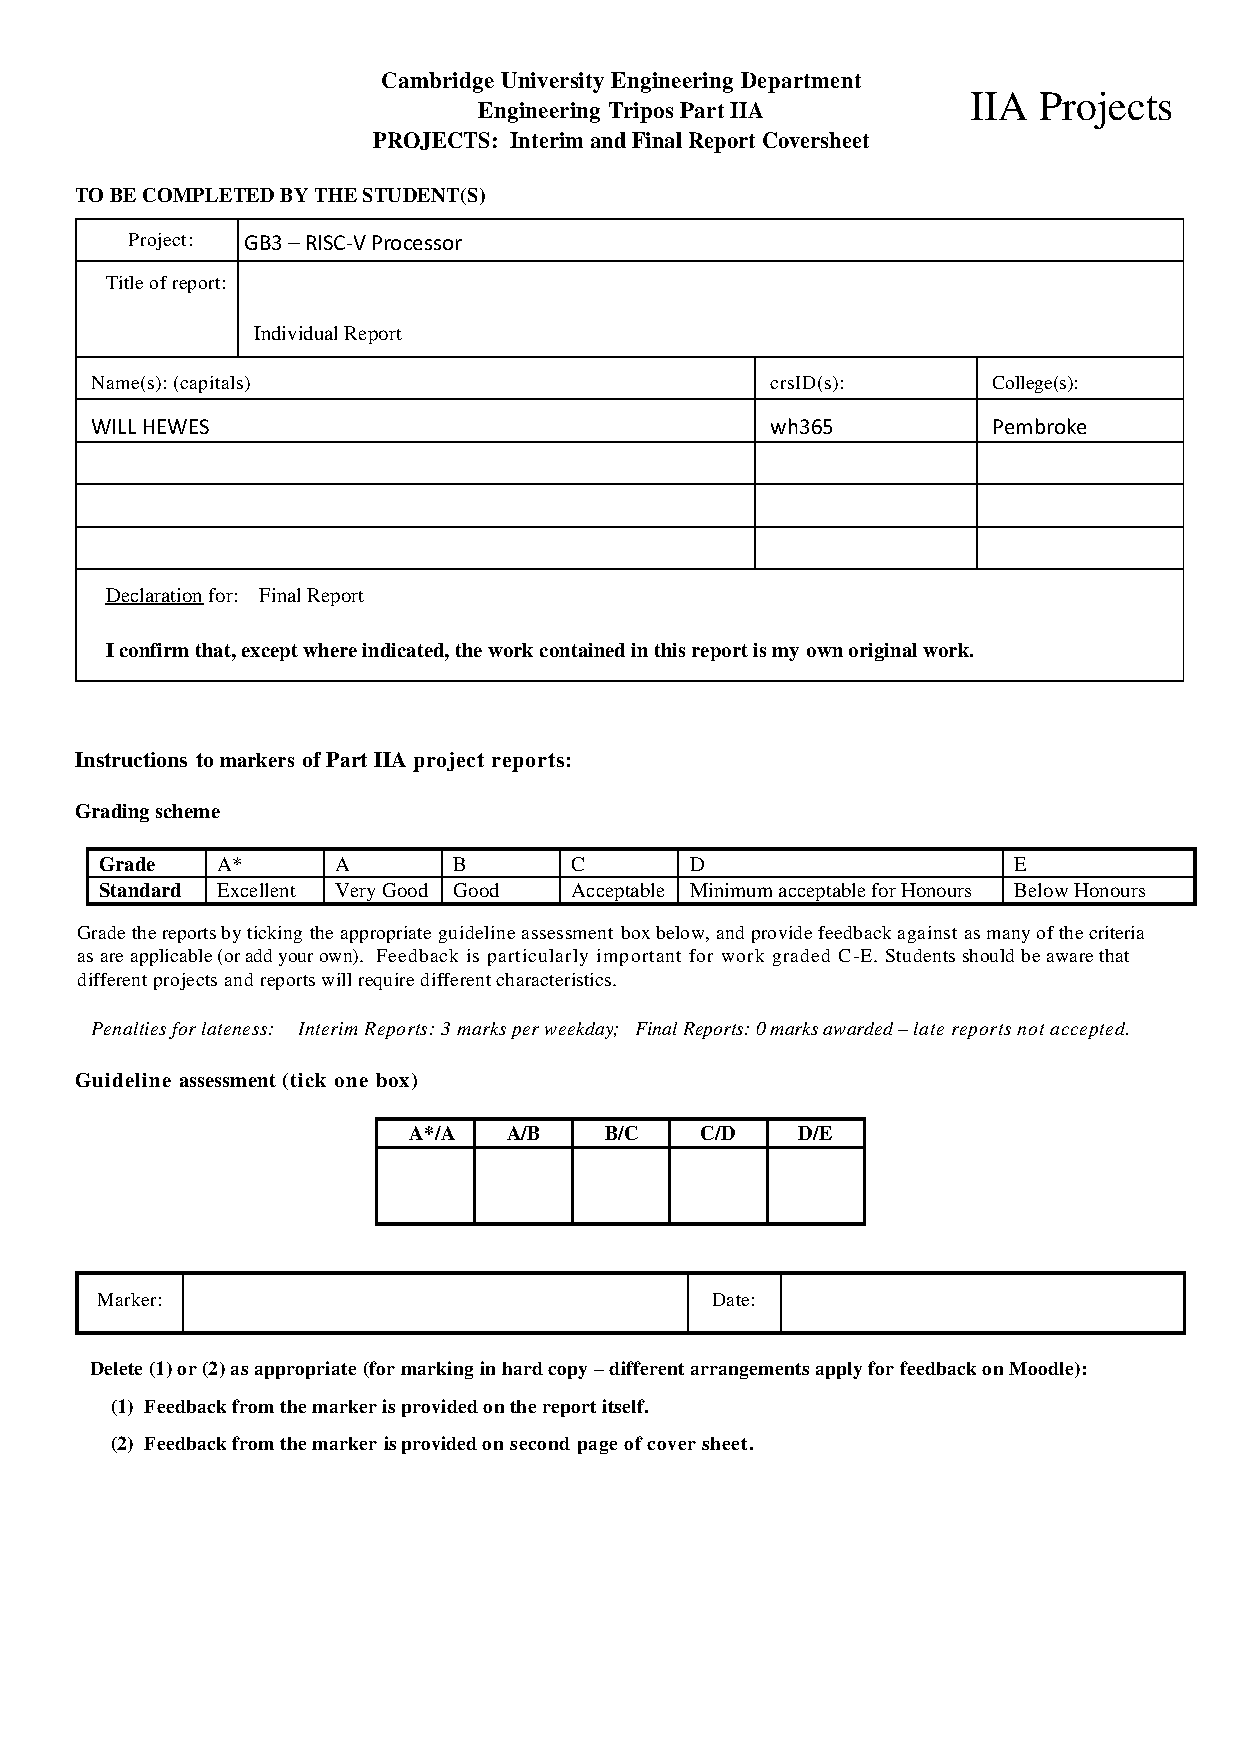
\includepdf[pages=-]{Handouts/IIA Project Coversheet Feedback Final Report.pdf}
\maketitle
\hrule
\tableofcontents
\newpage
\pagenumbering{arabic} \setcounter{page}{1}
% No more than 8 A4 sides, excluding appendices
% Include tables and descriptions in resource usage?

\section{Introduction}
\label{sec:Introduction}
% This section should give a detailed introduction to the changes
% you have implemented for your role on the team 
% (1 A4 side)

\section{Design Strategy}
\label{sec:Design_Strategy}
% Describing the specific design strategy employed for your role in the team (0.5-1 A4 side)
% Timeline diagram?
% Include subsection on the baseline processor, both description of its structure and resource usage

\section{Design Description}
\label{sec:Design_Description}
% For the components you implemented for your team (regardless of your role) (2-3 A4 sides)
% Include diagram on DSP blocks?
% Mention how your changes affect the other aspects
% Summarise original behaviour, describe original behaviour, justify it

\section{Problems Encountered}
\label{sec:Problems_Encountered}
% Problems encountered by you and their technical solutions (1-2 A4 sides)
% Maybe mention minimising the impact of the others contributions i.e. pipelining
% Warnings, missing reports, LED not blinking after some tests
% Inability to test LED always due to Cheng having it, less flexibility?

\section{Test Procedure}
\label{sec:Test_Procedure}
% Test procedure for your components in the team's efforts (1-2 A4 sides)
% Testing procedure automated flow
% Test on bubblesort and software
% Manual testing?
% Git version control helping to keep track of affects on resource usage etc., ease of use

\section{Conclusion}
\label{sec:Conclusion}
% Conclusions and recommendations for further improvements in your design and evaluation
% Use this section to provide a retrospective on how your team coordinated amongst yourselves
% how that worked, and what you would do differently in the future (1-2 A4 sides)

\newpage
\appendix
%Use this section to include diagrams, Verilog or C code, etc
\section{Resource Usage Data}

\begin{table}[H] 
    \centering
    \begin{tabularx}{0.6\textwidth}{X c c}
        \toprule
        Modification & LUTs & Block RAMs \\ \midrule
        Baseline $\rightarrow$ PC Gating & $9$ & $0$ \\
        PC Gating $\rightarrow$ CSR Removal & $159$ & $8$ \\
        CSR Removal $\rightarrow$ Signal Width Fix & $14$ & $0$ \\ \midrule
        \textbf{Total Reduction} & \textbf{$182$} & \textbf{$8$} \\
        \bottomrule
    \end{tabularx}
    \caption{Individual resource reductions following each modification}
    \label{tab:modification_reductions}
\end{table}


\begin{table}[H] 
    \centering
    \begin{tabularx}{0.65\textwidth}{X c c}
        \toprule
        Resource type & Used & \% of total \\ \midrule
        Logic cells (\texttt{ICESTORM\_LC}) & 3073 / 5280 & 58\,\% \\
        Block RAMs (\texttt{ICESTORM\_RAM}) & 20 / 30 & 66\,\% \\
        IO buffers (\texttt{SB\_IO}) & 8 / 96 & 8\,\% \\
        Global buffers (\texttt{SB\_GB}) & 5 / 8 & 62\,\% \\
        HF oscillators (\texttt{ICESTORM\_HFOSC}) & 1 / 1 & 100\,\% \\
        \bottomrule
    \end{tabularx}
    \caption{Baseline report}
    \label{tab:baseline}
\end{table}

\begin{table}[H] 
    \centering
    \begin{tabularx}{0.65\textwidth}{X c c}
        \toprule
        Resource type & Used & \% of total \\ \midrule
        Logic cells (\texttt{ICESTORM\_LC}) & 3064 / 5280 & 57\,\% \\
        Block RAMs (\texttt{ICESTORM\_RAM}) & 20 / 30 & 66\,\% \\
        IO buffers (\texttt{SB\_IO}) & 8 / 96 & 8\,\% \\
        Global buffers (\texttt{SB\_GB}) & 5 / 8 & 62\,\% \\
        HF oscillators (\texttt{ICESTORM\_HFOSC}) & 1 / 1 & 100\,\% \\
        \bottomrule
    \end{tabularx}
    \caption{Report after adding clock gating to the Program Counter module}
    \label{tab:Program_Counter}
\end{table}

\begin{table}[H] 
    \centering
    \begin{tabularx}{0.65\textwidth}{X c c}
        \toprule
        Resource type & Used & \% of total \\ \midrule
        Logic cells (\texttt{ICESTORM\_LC}) & 2905 / 5280 & 57\,\% \\
        Block RAMs (\texttt{ICESTORM\_RAM}) & 12 / 30 & 40\,\% \\
        IO buffers (\texttt{SB\_IO}) & 8 / 96 & 8\,\% \\
        Global buffers (\texttt{SB\_GB}) & 5 / 8 & 62\,\% \\
        HF oscillators (\texttt{ICESTORM\_HFOSC}) & 1 / 1 & 100\,\% \\
        \bottomrule
    \end{tabularx}
    \caption{Report after removing Control and Status Register (CSR) logic}
    \label{tab:CSR}
\end{table}

\begin{table}[H] 
    \centering
    \begin{tabularx}{0.65\textwidth}{X c c}
        \toprule
        Resource type & Used & \% of total \\ \midrule
        Logic cells (\texttt{ICESTORM\_LC}) & 2891 / 5280 & 57\,\% \\
        Block RAMs (\texttt{ICESTORM\_RAM}) & 12 / 30 & 40\,\% \\
        IO buffers (\texttt{SB\_IO}) & 8 / 96 & 8\,\% \\
        Global buffers (\texttt{SB\_GB}) & 5 / 8 & 62\,\% \\
        HF oscillators (\texttt{ICESTORM\_HFOSC}) & 1 / 1 & 100\,\% \\
        \bottomrule
    \end{tabularx}
    \caption{Report after removing unused control signal width}
    \label{tab:Signal_Width}
\end{table}

\end{document}